\documentclass[a4paper,12pt]{article} % тип документа

%  Русский язык
\usepackage[T2A]{fontenc}			% кодировка
\usepackage[utf8]{inputenc}			% кодировка исходного текста
\usepackage[english,russian]{babel}	% локализация и переносы

\usepackage{graphicx}               % импорт изображений
\usepackage{wrapfig}                % обтекаемые изображения
\graphicspath{{pictures/}}          % обращение к подкаталогу с изображениями
\usepackage[14pt]{extsizes}         % для того чтобы задать нестандартный 14-ый размер шрифта
\usepackage{amsfonts}               % буквы с двойными штрихами
\usepackage[warn]{mathtext}         % русский язык в формулах
\usepackage{indentfirst}            % indent first
\usepackage[margin = 25mm]{geometry}% отступы полей
\usepackage{amsmath}                % можно выводить фигурные скобочки -- делать системы уравнений
\usepackage[table,xcdraw]{xcolor}   % таблицы
\usepackage{amsmath,amsfonts,amssymb,amsthm,mathtools} % Математика
\usepackage{wasysym}                % ???
\usepackage{upgreek}                % ???  

\usepackage{caption}
\captionsetup{labelsep=period}
\usepackage{gensymb} % degree symbol

\begin{document}
	\begin{center}
		
		\normalsize{Федеральное государственное автономное образовательное учреждение высшего образования}
		
		\textbf{НАЦИОНАЛЬНЫЙ ИССЛЕДОВАТЕЛЬСКИЙ УНИВЕРСИТЕТ \\ <<МОСКОВСКИЙ ФИЗИКО-ТЕХНИЧЕСКИЙ ИНСТИТУТ>>}
		\vspace{13ex}
		
		\textbf{Лабораторная работа 2.1.2 \\ <<Определение $C_{p}/C_{v}$ методом адиабатического расширения>> }
		\vspace{40ex}
		
		\normalsize{Овсянников Михаил Александрович \\ студент группы Б01-001\\ 1 курс ФРКТ\\}
	\end{center}
	
	\vfill 
	
	\begin{center}
		г. Долгопрудный\\ 
		2021 г.
	\end{center}
	
	\thispagestyle{empty} % выключаем отображение номера для этой страницы
	
	\newpage

	\textbf{Цель работы:} определение отношения $C_{p}/C_{v}$ для воздуха по измерению давления в стеклянном сосуде. Измерения производятся сначала после адиабатического расширения газа, а затем после нагревания сосуда и газа до комнатной температуры.\\
	
	\textbf{В работе используются:} стеклянный сосуд; U-образный жидкостный манометр; резиновая груша.\\ 
	
	\section*{Экспериментальная установка.}
	
Используемая для опытов установка состоит из стеклянного сосуда А (объемом около 20 л), снабженного краном К, и U-образного жидкостного манометра, измеряющего избыточное давление газа в сосуде. Схема установки показана на рисунке 1.
	
	\begin{figure}[h!]
		\centering
		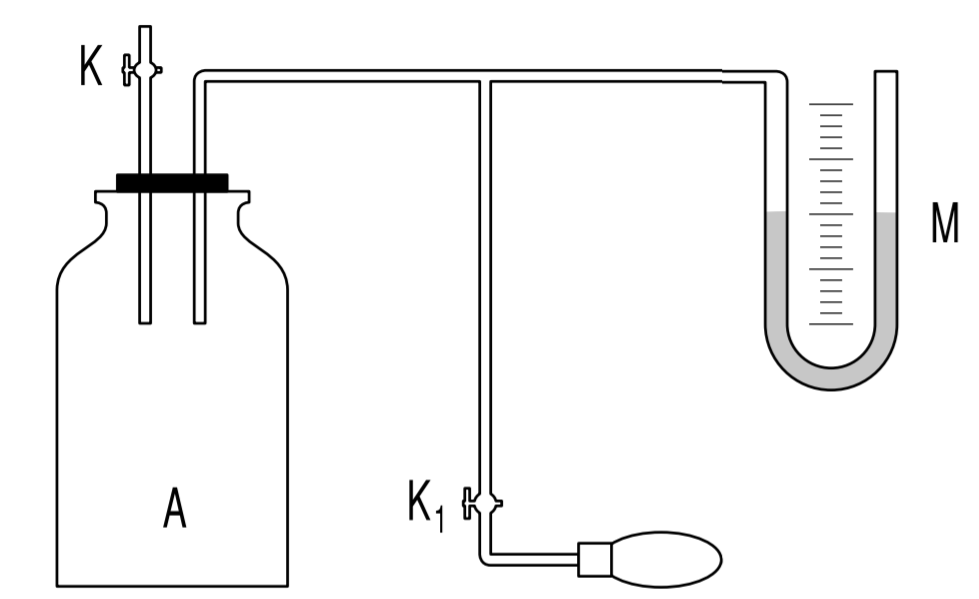
\includegraphics[scale = 0.4]{Pictures/Установка.png}
		\caption{Установка для определения $C_{p}/C_{v}$}
	\end{figure}

	
Избыточное давление воздуха создается с помощью резиновой груши, соединенной с сосудом трубкой с краном $\text{K}_{1}$.
	

В начале опыта в стеклянном сосуде А находится исследуемый газ при комнатной температуре $T_{1}$ и давлении $P_{1}$, несколько превышающем атмосферное давление $P_{0}$. После открытия крана К, соединяющего сосуд A с атмосферой, давление и температура газа будут понижаться. Это уменьшение температуры приближенно можно считать адиабатическим. Приближение основано на том, что равновесие в газах по давлению устанавливается намного быстрее, чем равновесие по температуре, которое происходит в процессе «диффузии тепла», диффузии интенсивности хаотического движения. Поэтому
	
	\begin{equation}
		\Delta t_{P} \ll \Delta t_{T},
	\end{equation}

\noindent	где $\Delta t_{P}$ и $\Delta t_{T}$ обозначают соответственно времена выравнивания давления и температуры.

	
 Выполнение условия (1) зависит, конечно, и от конструкции установки, в частности, от величины отверстия в кране К, которое должно быть достаточно большим. Ниже приведены численные оценки величин $\Delta t_{P}$ и $\Delta t_{T}$ и их влияния на точность опытов. Если открыть	кран К в течение такого промежутка времени $\Delta t$, что удовлетворяются условия
	
	\begin{equation}
		\Delta t_{P} \ll \Delta t \ll \Delta t_{T},
	\end{equation}
\noindent то теплообменом через стенки баллона можно приближенно пренебречь и считать процесс адиабатическим.


Преобразуем уравнение адиабаты с помощью уравнения Клапейрона к переменным $P, T$. Обозначим состояние газа после повышения давления в сосуде и выравнивания температуры с комнатной индексом «1», а состояние сразу после открытия крана и выравнивания давления с атмосферным — индексом «2». Получим

	\begin{equation}
		\left(\frac{P_{1}}{P_{2}}\right)^{\gamma - 1} = \left(\frac{T_{1}}{T_{2}}\right)^{\gamma}
	\end{equation}

Давление $P_{2}$ после адиабатического расширения газа равно атмосферному давлению $P_{0}$, а температура $T_{2}$ будет ниже комнатной температуры $T_{1}$ (температура газа понижается, так как работа расширения совершается за счет внутренней энергии газа).


После того как кран К вновь отсоединит сосуд от атмосферы, происходит медленное изохорическое нагревание газа со скоростью, определяемой теплопроводностью стеклянных стенок сосуда. Вместе с ростом температуры растет и давление газа. За время порядка $\Delta t_{T}$
система достигает равновесия, и установившаяся температура газа $T_{3}$ становится равной комнатной температуре $T_{1}$.


Изохорический процесс выравнивания температуры при закрытом кране подчиняется закону Гей-Люссака:

	\begin{equation}
		\frac{P_{2}}{T_{2}} = \frac{P_{3}}{T_{3}} = \frac{P_{3}}{T_{1}} 
	\end{equation}


\noindent Исключая с помощью (4) отношение температур $T_{1}/T_{2}$ из (3), найдем

	\begin{equation*}
			\left(\frac{P_{3}}{P_{2}}\right)^{\gamma} = 	\left(\frac{P_{1}}{P_{2}}\right)^{\gamma - 1}.
	\end{equation*}

\newpage
\noindent Отсюда учитывая, что $P_{2} = P_{0}$, находим $\gamma$:
	\begin{equation}
		\gamma = \frac{\ln{\left(P_{1}/P_{0}\right)}}{\ln{\left(P_{1}/P_{3}\right)}}
	\end{equation}


В нашем случае давления $P_{1}$ и $P_{3}$ отличаются от атмосферного на малую величину, измеряемую жидкостным U-образным манометром. Введем обозначения:
	\begin{equation*}
		P_{1} = P_{0} + \rho gh_{1}, \text{     } P_{3} = P_{0} + \rho gh_{2}.
	\end{equation*}

\noindent Разлагая логарифмы в ряд и пренебрегая членами второго порядка малости, получим

	\begin{equation}
		\gamma = \frac{\ln(1 + \rho gh_{1}/P_{0})}{\ln(1 + \rho gh_{1}/P_{0}) - \ln(1 + \rho gh_{2}/P_{0})} \approx \frac{h_{1}}{h_{1} - h_{2}}.
	\end{equation}

При желании можно произвести вычисления точно и определить, таким образом, величину ошибки, возникающей при использовании формулы (6).


Как следует из (6), для определения $\gamma$ необходимо знать избыточное (над атмосферным) давление в баллоне до адиабатического расширения газа и его избыточное давление после изохорного нагревания. Следует подчеркнуть, что обе величины должны измеряться в состоянии термодинамического равновесия, т. е. после прекращения теплообмена. Для этого необходимо закрыть кран К после установления в сосуде атмосферного давления, но еще до того, когда там начнется нагревание газа. То есть нужно выполнить условия (2). 


\textbf{Время вытекания газа.} Оценим время выравнивания давления $\Delta t_{P}$, пренебрегая вязкостью газа. В данном случае это можно сделать из-за малой длины трубки, через которую вытекает газ.


После открытия крана К по газу со скоростью звука $c$ будет распространяться волна разрежения и через время $L/c$ (где $L$ — высота сосуда) она достигнет дна. Весь газ придет в движение и через несколько таких интервалов процесс вытекания будет почти установившимся, квазистационарным. При этом скорость истечения v можно рассчитать по уравнению Бернулли для несжимаемой среды, поскольку давление воздуха мало отличается от атмосферного и изменением плотности допустимо пренебречь:

	\begin{equation*}
		v = \sqrt{2(P - P_{0})/\rho_{0}}
	\end{equation*}


За время $dt$ из сосуда через отверстие площадью $S_{r}$ вытечет масса газа $\rho_{0}S_{r}vdt$, где плотность взята при атмосферном давлении из-за малого изменения давления газа.


В сосуде объема $V_{0}$ давление за это же время снизится на $dP$, и масса газа при адиабатическом истечении уменьшится на величину

	\begin{equation*}
		dm = V_{0}d\rho = \frac{V_{0}}{c^2}dP.
	\end{equation*}

\noindent Здесь использовано определение адиабатической скорости звука

	\begin{equation*}
		c^2 = \left(\frac{\partial P}{\partial \rho}\right)_{S}.
	\end{equation*}


Составив баланс вытекающей массы и остающейся в сосуде, получим дифференциальное уравнение:

	\begin{equation*}
		\frac{dP}{\sqrt{P - P_{0}}} = -\frac{\sqrt{2\rho_{0}}S_{r}c^2}{V_{0}}dt
	\end{equation*}


Интегрируя, найдем искомое время вытекания газа:

	\begin{equation}
		t_{P} = \frac{V_{0}}{S_{r}c}\sqrt{\frac{2(P - P_{0})}{\gamma P_{0}}}.
	\end{equation}


Для численной оценки используем приблизительные данные установки: диаметр сосуда 25 см, диаметр отверстия 1 см, $L = $50 см $c = 340$ м/с, $\gamma  = 1,4 $, $P - P_{0}$ = 10 см водяного столба. Из (7) найдем $t_{P} = 0,1$ с.


За рассчитанное время вытекания газа из сосуда звуковая волна может 34 раза пройти от отверстия до дна и обратно. Этого достаточно, чтобы течение считать квазистационарным и применять уравнение Бернулли.


Отметим, что после выравнивания давления из-за инерции вытекающей струи могут происходить колебания воздуха в сосуде как в акустическом резонаторе. Поэтому при малых временах открытия крана $\Delta t$ t (меньше одной секунды) результаты отдельных измерений заметно отличаются друг от друга (случайный разброс вызван не только колебаниями, но и неопределенностью во времени открытия крана). При увеличении времени $\Delta t$ (больше одной секунды) колебания давления из-за затухания благодаря вязкости становятся меньше, но за большее время увеличивается теплообмен. Следствием является уменьшение давления $P_{3}$ и занижение значения $\gamma$.


\noindent \textbf{Нагревание газа от стенок сосуда.} Перейдем к оценке теплообмена между газом и стенками за время выравнивания давления, то есть примерно за 0,5 с. За такое время глубина прогревания невелика, значительно меньше размеров сосуда, поэтому нагревание приближенно можно считать одномерным. Процесс изменения температуры в пространстве и времени описывается уравнением теплопроводности (в частных производных), точное решение которого сложно даже для одномерного случая. Поэтому ограничимся оценкой.


Все физические свойства среды, влияющие на исследуемый процесс, отражены в уравнении теплопроводности всего через один параметр — коэффициент температуропроводности $\chi = \varkappa / (\rho c_{p})$, где $\varkappa$ - коэффициент теплопроводности, $c_{p}$ — теплоемкость при постоянном давлении единицы массы газа, $\rho$ — его плотность. Размерность $\chi$ в системе СИ есть $\text{м}^2/\text{c}$.


Если в начальном распределении температуры нет постоянных с размерностью длины, как, например, при нагревании полупространства от горячей стенки, то решение может быть функцией только от одного безразмерного параметра $x^2/(\chi^t)$, где $x$ - координата, $t$ — время (такое решение называется автомодельным). Одному и тому же значению этого параметра будет соответствовать одна и та же температура, положение которой в пространстве меняется. Расстояние от стенки до точки с любой заданной температурой увеличивается пропорционально квадратному корню из времени. При $x^2/(\chi ^t) = 1$, то есть при $x = \sqrt{\chi ^t}$, в точном решении задачи о нагревании полупространства, температура равна примерно среднему значению между постоянной температурой горячей стенки и температурой первоначально холодной теплопроводящей среды. Это значение $x$ можно использовать для оценки толщины слоя газа, нагревшегося от стенки сосуда при предполагаемом его адиабатическом охлаждении, сопровождающим процесс вытекания.


В соответствии с оценкой времени вытекания газа из сосуда примем для определения влияния теплопроводности время $t = 0,5$ с. Для воздуха $c_{p} = 0,99$ Дж/(г$\cdot$K), $\rho = 1,29$ кг/м$^3$, $\varkappa = 2,50 \cdot 10^{-2}$ Вт/(м$\cdot$К). По этим данным $\chi = 0,19$ см$^2/$с,
и при $t = 0,5$ с глубина нагревания составит $x = 0,3$ см.


При радиусе сосуда $R = 12,5$ см доля неохлажденного воздуха из-за контакта со стенкой сосуда составит, согласно приведенной оценке, $2\pi Rx/(\pi R^2)$ = 0,05 то есть 5 \% от массы газа в сосуде. Следовательно, давление $P_{3}$ и величина $h_{2}$ будут во столько же раз меньше, что приведет к уменьшению величины $\gamma$ в соответствии с формулой (6) в $[h_{1}/(h_{1} - h_{2})] \cdot 0,05$ раз. Например, при $h_{1} = 20$ см и $h_{2} = 10$ см уменьшение $\gamma$ по этой причине составит также 5\%. Это довольно много, так как разница между $\gamma$ двухатомного (1,40) и многоатомного (1,33) газа по классической теории теплоемкости также составляет всего 5\%. Приведенная оценка ошибки может быть несколько уменьшена, если учесть охлаждение стеклянных стенок сосуда.

\newpage
\noindent \textbf{Охлаждение стенок.} Глубину охлаждения стенок сосуда за время вытекания газа можно оценить аналогичным способом.


Для стекла теплоемкость $c = 1,0$ кДж/(кг$\cdot$К), плотность $\rho = 2,5 \cdot 10^3$ кг/м$^3$, теплопроводность $\varkappa = 1,0$ Вт/(м$\cdot$К). По этим данным получим $\chi = 0,4 \cdot 10^{-2}$ см$^2$/с и глубина охлаждения получится равной всего 0,045 см.


Из полученной оценки следует, что глубина охлаждения стекла примерно в семь раз меньше, чем глубина нагревания воздуха за то же время. Если учесть, что теплоемкость стекла на единицу объема на три порядка больше теплоемкости воздуха, то получится, что изменение температуры стенок будет примерно в сто раз меньше, чему газа. Оценка ошибки остается прежней, учет охлаждения стекла в данном случае не оказывает заметного влияния на нагревание воздуха.


Из приведенных оценок теплопередачи следует, что она может оказывать существенное влияние на измеряемые величины, следствием чего является заниженное значение измеренной величины показателя адиабаты. Поэтому рекомендуется многократное проведение эксперимента при разных временах открытия крана, а затем интерполяция и экстраполяция полученных значений.

\newpage
\section*{Ход работы}

\begin{enumerate}
	\item Перед началом работы убедимся, что краны и места сочленений трубок достаточно герметичны. Для этого наполним баллон воздухом до давления, превышающего атмосферное на 10–25 см вод. ст., и перекроем кран $\text{K}_{1}$. Увеличение давления в баллоне сопровождается повышением температуры. Вследствие теплопроводности стенок с течением времени происходит понижение температуры воздуха в баллоне и вместе с тем понижение давления (изохорное охлаждение). По U-образному манометру снимем зависимость $h$ высоты правого столба жидкости от времени $t$ (таблица 1) и построим график $h = f(t)$, чтобы найти время установления $\Delta t_{T}$ (график 1).
	
	
	\begin{table}[h!]
		\centering
		\begin{tabular}{|c|c|c|c|c|c|c|c|c|}
			\hline
			$t$, c  & 0   & 5   & 10  & 20  & 30  & 40  & 50  & 60  \\ \hline
			$h$, см & 7,8 & 7,9 & 8,0 & 8,1 & 8,1 & 8,2 & 8,2 & 8,2 \\ \hline
		\end{tabular}
	\caption{}
	\end{table}

	\begin{figure}[h!]
		\centering
		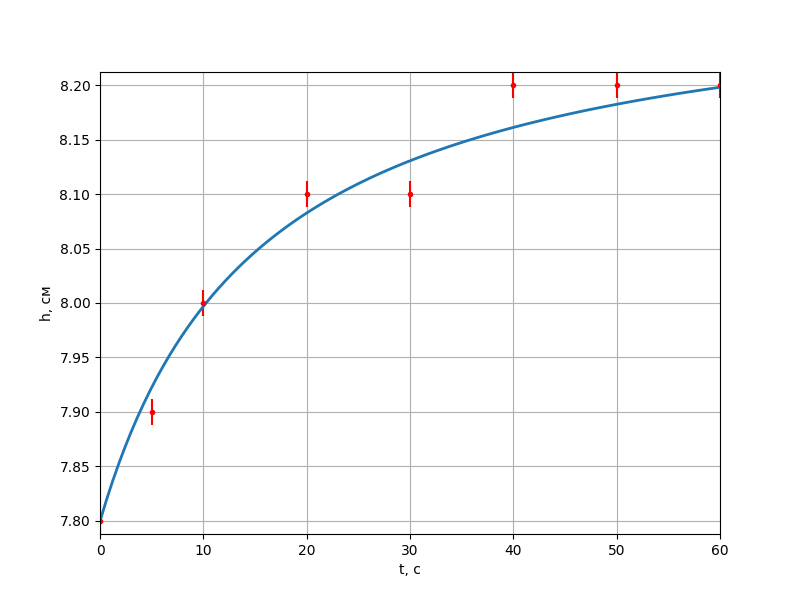
\includegraphics[scale = 0.8]{Pictures/h(t).png}
		\caption*{График 1}
	\end{figure}
\newpage
График является аппроксимацией вида $y = a + \frac{b}{(cx+d)^{e}}$ с коэффициентами, полученными при помощи МНК.


Из графика 1 видно, что время установления $\Delta t_{T} \thicksim 60 $ c.


\item Запишем разность уровней жидкости в манометре $h_{1}$. Откроем на короткое время кран К и закроем его снова. Подождем, пока уровень жидкости в манометре перестанет изменяться. Это произойдет, когда температура газа в сосуде сравняется с комнатной, примерно через время $\Delta t_{T}$. Запишем разность уровней жидкости в манометре $h_{2}$.  Проведем 8 таких измерений, каждый раз вновь заполняя сосуд, выжидая время установления уровня $h_{1}$, а затем открывая кран К примерно на $\Delta t = 0,5$ с. Затем делаем 8 измерений с интервалом времени 5 с. При каждом опыте записываем значения $h_{1}$ и $h_{2}$ после того, как уровни перестанут изменяться. По полученным данным вычислим согласно формуле (6) соответствующие величины $\gamma$. Все эти результаты запишем в таблицу 2.

\begin{table}[h!]
	\centering
	\begin{tabular}{|c|c|c|c|c|c|c|c|c|}
		\hline
		$t$, с      & 5    & 10   & 15   & 20   & 25   & 30   & 35   & 40   \\ \hline
		$h_{1}$, см & 22,6 & 21,8 & 21,1 & 22,4 & 24,2 & 24,2 & 25,9 & 23,3 \\ \hline
		$h_{2}$, см & 5,6  & 4,8  & 4,1  & 3,4  & 2,8  & 2,2  & 1,7  & 1,2  \\ \hline
		$\gamma$    & 1,329 & 1,282 & 1,241 & 1,179 & 1,130 & 1,100 & 1,070 & 1,054 \\ \hline
	\end{tabular}
\caption*{Таблица 2}
\end{table}

\newpage
Построим график $\gamma(t)$.

$\sigma_{\gamma} = \gamma \sqrt{\left(\frac{\sigma_{h_{1}}}{h_{1}}\right)^2 + \left(\frac{\sigma_{h_{1} - h_{2}}}{h_{1} - h_{2}}\right)^2}$;  \hspace{30mm}   $\sigma_{h_{1}} = \sigma_{h_{2}} = \sigma_{h} = 0,1$ см.
\vspace{7mm}

$\sigma_{h_{1} - h_{2}} = \sqrt{\sigma_{h_{1}}^2 + \sigma_{h_{2}}^2} = \sqrt{2}\sigma_{h}$.


Ошибка каждого значения $\gamma$ составляет $\thicksim 0,012$, поэтому используем МНК.

\begin{figure}[h!]
	\centering
	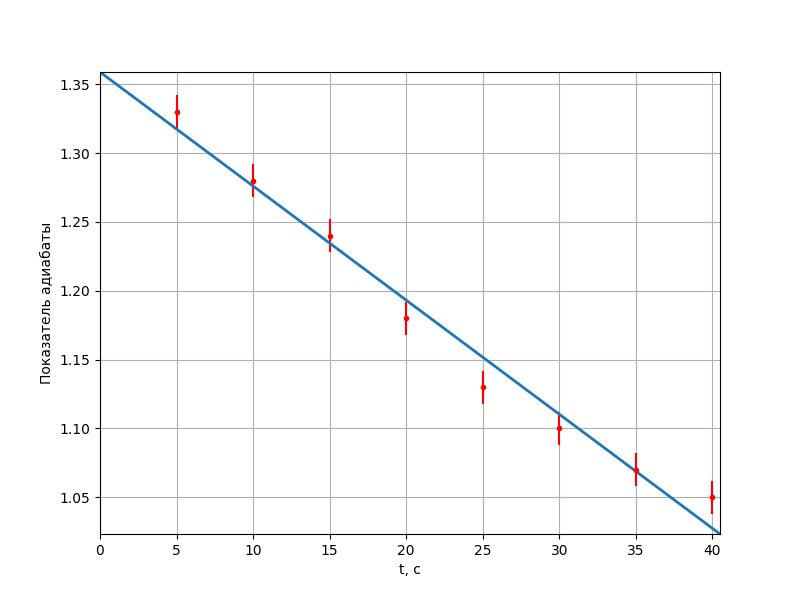
\includegraphics[scale=0.8]{Pictures/g(t).png}
	\caption*{График 2}
\end{figure}

\item Окончательный результат следует получить экстраполяцией зависимости $\gamma$ от $t$ примерно к значению $t = 0,15$ c, когда давление уже почти сравнялось с атмосферным, но теплопроводность еще не так сильно повлияла на уменьшение $\gamma$.


Получаем $\gamma = \gamma_{(0,15)} = 1,358$.
\newpage
\item Оценим ошибку измерений.

По МНК было получено наилучшее уравнение:


$\gamma = kt + b = -0,0083t + 1,359$.


$\sigma_{\gamma(0,15)} = \sqrt{\sigma_{k}^2 t^2 + \sigma_{b}^2}$.


По МНК было получено $\sigma_{k} = 0,0004 \text{ c}^{-1}$, $\sigma_{b} = 0,046$.


$\sigma_{\gamma(0,15)} = \sqrt{\sigma_{k}^2 t^2 + \sigma_{b}^2} = 0,046$.


Окончательно имеем:

$\gamma = (1,358 \pm  0,046)$.



\end{enumerate}
\section*{Вывод}

В работе пронаблюдались процессы адиабатического расширения и изохорического нагревания воздуха. Был определен показатель адиабаты для воздуха $\gamma = (1,358 \pm 0,046)$. Ошибки вызваны недостаточной точностью приборов и несовершенством техники измерения.
\end{document}
